\flchap{Evaluation}
\label{chap:eval}

We evaluate the system against a baseline implementation, and we investigate
several modifications to the system.
%
We use five-fold cross validation on the target users to evaluate the system.
We evaluated the FriendlyLocation system against the 249,584 target users.

For each of the folds, we ran the tree classifier and generated a new set of
curves for $\pContact$ from the training data.
%
We did not recalculate $\pStrangers$ or the probability as a function of distance
used for the baseline, since these are fairly independent of the selected set
of users.

We evaluate the system against the metrics used in previous works:
accuracy at 25 miles (ACC) which was used in \cite{backstrom2010find}
and average error distance (AED) proposed in \cite{cheng2010you} and
extended in \cite{li2012towards}.
%
Following the notational conventions from \cite{li2012towards}, we define ACC
and AED for a set of users $u \in U$ with $\Err(u)$ as the distance between a
target user's home location and the predicted location.

Accuracy is the fraction of users who live within 25 miles of their predicted
location:
\[
    \ACC(U) = { |\{ u \in U : \Err(u)\le25 \}| \over |U| }
\]

Average error distance (reported as AED@100\%) is as follows:
\[
    \AED(U) = { \sum_{u \in U} \Err(u) \over |U| }
\]

We also use the extension of AED created by \cite{li2012towards}:
\begin{quote}
However, as AED is easily affected by outliers in results, we report AED at
different percentiles (60\%, 80\% and 100\%) of users ranked by their error
distances. E.g., AED@60\% is the average error distance of the top 60\% of
users ranked by their error distances.
\end{quote}
The effect of outliers that they mention is even larger in our work than theirs
because we are using locations from around the world instead of focusing on
just the U.S.

We investigate several implementations of the FriendlyLocation system along
with two baseline systems, which we will discuss in upcoming sections:
\begin{description}
\item[Baseline] This is based on the MLE estimator presented in
    \cite{backstrom2010find}. Some changes to the system had to be made to make it
    work on Twitter's directed graph. (Facebook friendships are always
    reciprocal.)
\item[Nearest Contact] This predictor chooses the location of the contact that
    the tree regressor picks as the closest contact.
\item[FriendlyLocation Basic] This is the system described in the previous
    section with only information from the locations of contacts.
\item[FriendlyLocation - Strangers] This is the system described in the previous
    section without $\pStrangers$.
\ifdefined\THESIS
\item[FriendlyLocation + Time Zone] This is the system described in the previous
    section plus the target user's time zone information.
\fi
\item[FriendlyLocation + Location] This is the system described in the previous
    section plus the target user's reported location is included in the
    estimation.
\end{description}

\begin{figure}[tb]
\centering
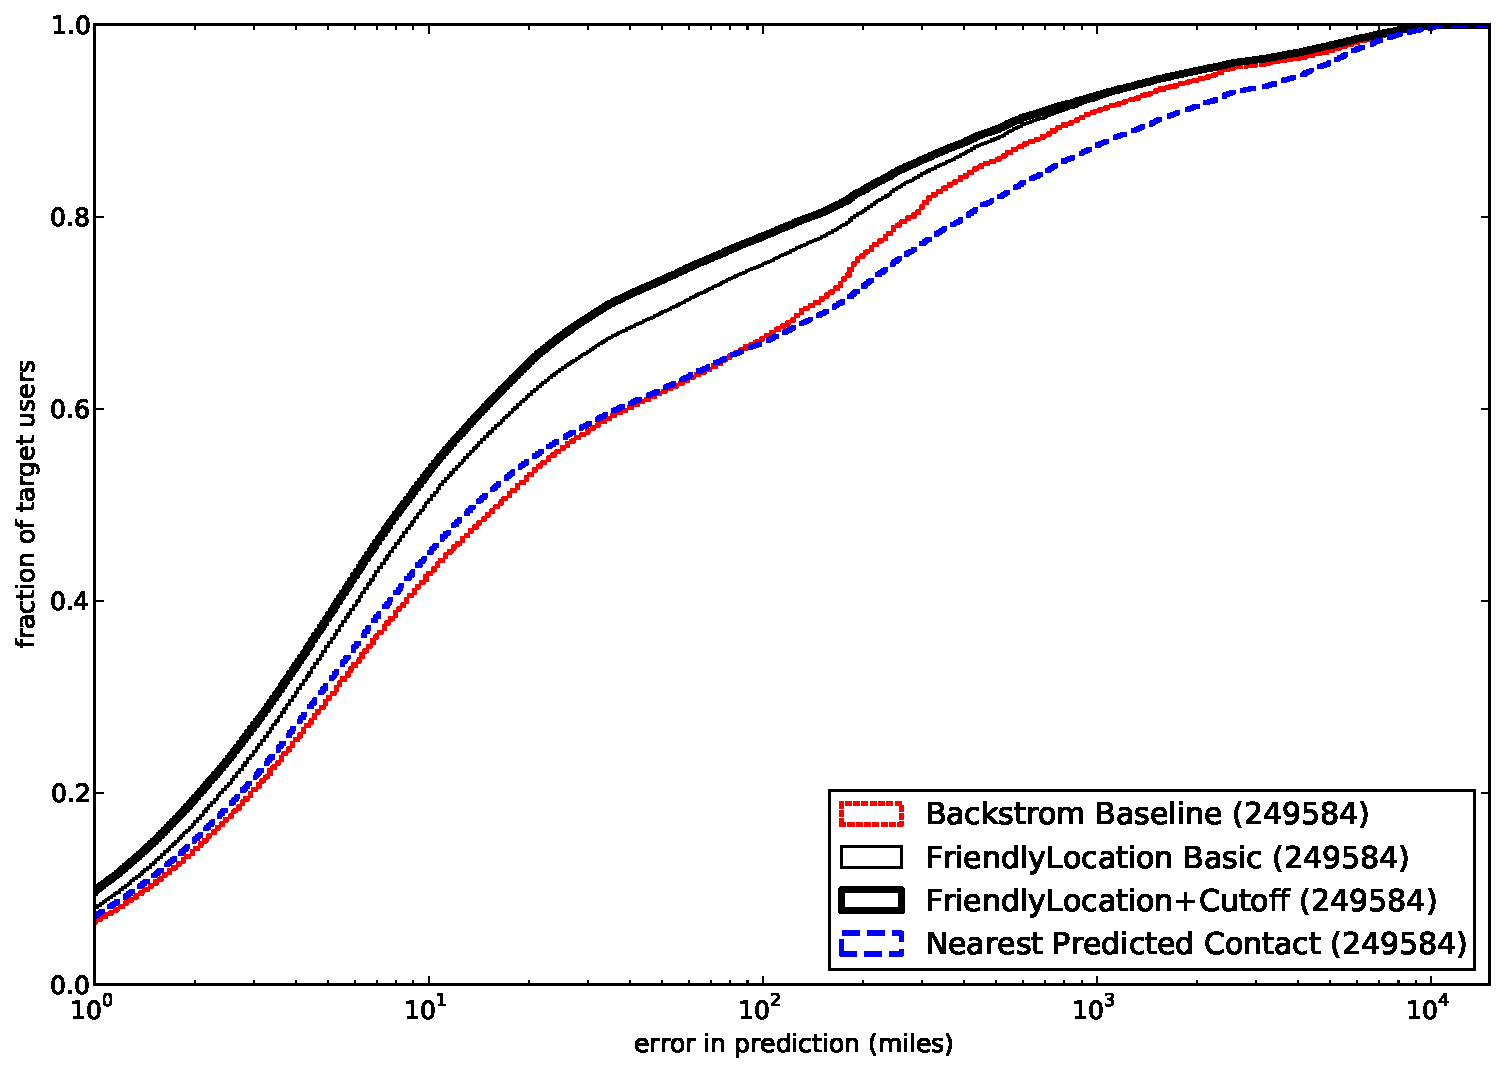
\includegraphics[width=\linewidth]{figures/fl_basic.pdf}
\caption{
    FriendlyLocation against several baseline systems.
}
\label{fig:results}
\end{figure}

\begin{table*}[tb]
\centering
\begin{tabular}{l  r r r r}
    Model & aed@60 & aed@80 & aed@100 & acc@25 \\
    \hline
    Baseline & 8.41$\pm$.038 & 40.8$\pm$.20 & 426$\pm$3.9 & 55.7\%$\pm$.09\% \\
    Nearest & 7.73$\pm$.117 & 50.3$\pm$.39 & 594$\pm$9.3 & 56.5\%$\pm$.22\% \\
    FriendLoc$-$Strangers & 5.79$\pm$.028 & 25.2$\pm$.18 & 377$\pm$4.3 & 62.4\%$\pm$.09\% \\
    FriendLoc Basic & 5.35$\pm$.008 & 21.4$\pm$.12 & 364$\pm$3.2 & 63.9\%$\pm$.05\% \\
\ifdefined\THESIS
    FriendLoc+Time Zone & 5.33$\pm$.009 & 21.1$\pm$.07 & 352$\pm$3.5 & 64.0\%$\pm$.04\% \\
\fi
    FriendLoc+Location & 4.54$\pm$.011 & 15.7$\pm$.27 & 325$\pm$2.6 & 66.9\%$\pm$.16\% \\
    FriendLoc+Cutoff & 4.56$\pm$.026 & 15.1$\pm$.22 & 343$\pm$4.2 & 67.4\%$\pm$.08\% \\
\end{tabular}
\caption{
    Results of our location prediction system when compared to a baseline.
    The value after the $\pm$ is the standard deviation from the five-fold
    cross-validation.
    Including the target user's time zone information does not improve the
    results, but using the target user's reported location, if they gave one,
    makes for significantly better results.
}
\label{tab:results}
\end{table*}

\flsec{Basic FriendlyLocation}

Table~\ref{tab:results} shows our system compared to a baseline implementation.
%
As seen in the table our basic FriendlyLocation system predicts the location
within 25 miles 63.9\% of the time.
%
Our basic system preforms significantly better than the baseline implementations.
%
The results are more impressive when you look at it in terms of average error
distance.
%
The baseline system has an average error distance of 40.8 for the best 80\% of
predictions, and our basic system has an average error distance of 21.4.
%
This means that our system is better at making good estimates better than it is
at making bad estimates good.
%
Unfortunately, when the predictor is wrong, it can be very wrong.
%
As seen in Figure~\ref{fig:results}, around a tenth of the predictions are worse
than 1000 miles for all of the predictors.
%
Some of this inaccuracy may be caused by inaccurate training data, but there is
no real way to know.

\jam{Do we want to include the omniscient predictor that magically picks the
closest contact?
%
The comparison to the omniscient predictor shows that there is room for improvement.
%
Many users who have an incorrectly predicted location have at least one contact
that is closer than the incorrectly predicted location.
}

\ifdefined\THESIS
\flsec{Time Zone}
When the predictor is wrong, it is often wrong by thousands of miles.
%
All users on Twitter have a time zone setting for their account which is used
to display the times that tweets were posted.
%
The time zone is set automatically when a user registers, and the user can
change it, but it is still not always correct.
%
The time zone information is made available on the Twitter API as the offset
in seconds from UTC.
%
We compared the longitudes of the target users to the UTC offset for their
profiles.
%
We put the target users into one of 24 groups based on x, the target user's
longitude and z, the UTC offset measured in hours:
${(\lfloor {x\over15}\rfloor-z+24)\mod{24}}$.
%
We found that 72\% of Twitter users fit into either group 0 or 1.
%
We define $\pTimeZone$ to be the fraction of the target users who fit into one
of the 24 groups.
%
We modified the formula for $\FriendLoc$ to include $\pTimeZone$ as follows and
re-ran the evaluation.
\[
    \pTimeZone(l,z)
    \left(
        \prod_{l^c_k \in L,p_k \in P}
        {\pContact(\quantile(p_k),|l-l^c_k|) \over (1-p(|l-l^c_k|))}
    \right)
    \pStrangers(l)
\]
The evaluation results for this formula are in the ``FriendLoc+Time Zone'' row
of Table~\ref{tab:results}.
%
We hoped that the time zone would help us avoid locations on the wrong side of
the world; unfortunately, adding the time zone information does not improve the
location prediction.
%
Part of the problem is that the time zone settings are often wrong---over 9\% of
the target users have a time zone setting in the hemisphere opposite their home
location.
%
The actual time zones on the earth have lines that are much more complex than
the simple metric we used, but they rarely differ by more than an hour one way
or the other.
%
Since this showed so little benefit, it is unlikely to be improved by better
time zone lines.
\jam{Do we want the time zone section?}
\fi

\flsec{Location Field}
Many Twitter users fill out the text-based location field.
%
If this user-reported data is good, there is no reason to spend time
crawling their contacts.
%
It would be nice to use this information when predicting location, but
the target users we used to do the evaluation are less concerned about
the privacy of their location information than the average Twitter user.
%
As a result, they tended to give more precise information in the location
field of their user profile than other users.
%
We assume that the locations supplied by the contacts are more
representative of normal Twitter users so we added noise to the locations
of the target users to make the distribution of the quality of their
locations would match the quality of the contacts.
%
First, we sorted all the target users and all the contacts by their
PLE(predicted location error).
%
Next, we looked at each percentile of the target users and compared
their PLE to the PLE for that percentile in the contacts.
%
For each of the target users, we moved the user's location based on
reverse geocoding away from the user's actual median location based on the
difference between the PLEs.
%
For example, the median PLE for a target user was 5.9 miles, and the median
PLE for a contact was 6.7 miles.
%
This means that we need to add .8 miles of noise to a target user
with a PLE of 5.9 so that the quality of the geo-located target user's location
would match the quality of normal Twitter users.
%
We also removed the location field from 17\% of the target users to
make the proportion of target users with a location match the general
Twitter population.

After doing this, we can use the user-supplied location of the user we are
going to predict.
%
We investigate two different ways of using this information.
%
The simpler of the two, which we refer to as ``FriendLoc+Cutoff'' in
Table~\ref{tab:results}.
%
If the PLE for the target user's geocoded location is less than or equal to 25
miles, then we use the geocoded location as the actual location; otherwise, we
ignore the geocoded location and just use $\FriendLoc$t diff to find the location.
%
This method locates 67.4\% of users within 25 miles, and is the best method
that we found.

We also look at including the geocoded location in the maximum-likelihood
estimation similar to what we did for time zones.
%
The same data that was used to generate Figure~\ref{fig:DiffMlocMdist} can be
used to calculate the probability that a user lives a certain distance from
their geocoded location.
%
We take the location error, which is the distance between a user's home
location and geocoded location, for all the target users with a location the
geocoder can decode, and find the distribution of these errors.
%
This lets us add $\pLocation$ into the maximum-likelihood estimator:
\[
    \pLocation(|l-l^g|)
    \left(
        \prod_{l^c_k \in L,p_k \in P}
        {\pContact(\quantile(p_k),|l-l^c_k|) \over (1-p(|l-l^c_k|))}
    \right)
    \pStrangers(l)
\]
\jam{Do we want ``FriendLoc+Location''? It helped, but it is not as good as the
    cutoff and more complicated.}


\flsec{Ignoring Strangers}
Calculating $\pStrangers$ is very expensive.
%
It only has to be computed once, but if you wanted to do location prediction on
a different social network, it would need to be recomputed.
%
We investigate the FriendlyLocation system without this information, by running
prediction without multiplying by $\pStrangers$ when calculating the overall
probability for each location:
\[
    \prod_{l^c_k \in L,p_k \in P} \pContact(\quantile(p_k),|l-l^c_k|)
\]
As seen in Table~\ref{tab:results}, removing this information results in a
slightly worse prediction.
%
There is a trade-off to be made here, and it may not be worth the time it takes
to calculate $\pStrangers$.

\flsec{Random Bits}

\jam{do we want to do us-only evaluation?}

\jam{ Although we limited the crawler to 25 randomly-picked contacts per target
user, if FriendlyLocation is going to be used as part of a larger system, the
crawler should pick users based on relationship type before crawling.}
